\section{Implementacja}
\label{sec:implementacja}

Rozdział opisuje program, którym przeprowadzono wszystkie eksperymenty: podział na warstwę obliczeniową i warstwę prezentacji, sposób przechowywania wag, dyskretną wersję reguły Oji, symulację dynamiki i wizualizację kolejnych kroków. Na końcu podano, jak zapewniono powtarzalność wyników.

\subsection{Architektura}
\label{sec:architektura}

Program składa się z dwóch warstw. Warstwa obliczeniowa, napisana w języku Rust, to jedno narzędzie wiersza poleceń \texttt{compute} z podpoleceniami wymienionymi w Tabeli~\ref{tab:podpolecenia}. Każde uruchomienie czyta konfigurację z pliku TOML, a wyniki zapisuje do plików: małe podsumowania w formacie JSON, tabele prób w formacie Parquet, a wagi, zbiory wzorców i historie stanów w binarnym formacie NumPy (\texttt{.npy}). Warstwa prezentacji, napisana w Pythonie, to pakiet \texttt{hopfield-analysis}, który tylko czyta te pliki i rysuje wykresy. Wszystkie liczby podane w raporcie pochodzą więc z warstwy obliczeniowej, a rysunki można odtworzyć bez ponownych obliczeń. Przepływ danych pokazano na Rysunku~\ref{fig:przeplyw}.

\begin{figure}[H]
    \centering
    \ifrysunki
    \begin{tikzpicture}[
        box/.style={draw, rounded corners=2pt, align=center, font=\small, text width=2.2cm, minimum height=1.1cm},
        arrow/.style={-{Latex[length=2mm]}},
        node distance=0.55cm,
    ]
        \node[box] (config) {konfiguracja\\TOML};
        \node[box, right=of config] (compute) {\texttt{compute}\\(Rust)};
        \node[box, right=of compute] (results) {wyniki\\JSON, Parquet,\\\texttt{.npy}};
        \node[box, right=of results] (analysis) {\texttt{hopfield-}\\\texttt{analysis}\\(Python)};
        \node[box, right=of analysis] (figures) {rysunki\\PDF, PNG};
        \node[box, above=0.45cm of compute] (datasets) {zbiory wzorców\\CSV, \texttt{.npy}};
        \draw[arrow] (config) -- (compute);
        \draw[arrow] (datasets) -- (compute);
        \draw[arrow] (compute) -- (results);
        \draw[arrow] (results) -- (analysis);
        \draw[arrow] (analysis) -- (figures);
    \end{tikzpicture}
    \fi
    \caption{Przepływ danych między warstwą obliczeniową i warstwą prezentacji.}
    \label{fig:przeplyw}
\end{figure}

\begin{table}[H]
    \centering
    \caption{Podpolecenia narzędzia \texttt{compute}.}
    \label{tab:podpolecenia}
    \small
    \begin{tabularx}{\textwidth}{>{\ttfamily}l X}
        \toprule
        \normalfont Podpolecenie & Przeznaczenie \\
        \midrule
        inspect & podgląd zbioru wzorców: wymiary, statystyki i nakładania \\
        convert-images & konwersja zdjęć na bitmapy o pikselach $\pm 1$ \\
        generate & tworzenie zbiorów z grupami podobnych wzorców \\
        train & uczenie sieci i zapis wag oraz stabilności wzorców \\
        recall & pojedyncze odtwarzanie z zapisem wszystkich odwiedzonych stanów \\
        experiment & siatka zbiorów, reguł, trybów i poziomów uszkodzenia z wieloma próbami \\
        capacity & stabilność wzorców przy rosnącej liczbie wzorców \\
        search-stable & wyszukiwanie licznego zbioru bitmap \mbox{5x5}, które są stabilne \\
        benchmark & pomiar czasu i pamięci uczenia oraz odtwarzania w funkcji $N$ \\
        \bottomrule
    \end{tabularx}
\end{table}

\subsection{Przechowywanie wag}
\label{sec:wagi}

Sieć przechowuje wagi na jeden z dwóch sposobów. Wagi gęste to pełna macierz $N \times N$ liczb zmiennoprzecinkowych podwójnej precyzji, która zajmuje $8N^2$ bajtów. Dla bitmap o wymiarach \mbox{300x200}, czyli $N = \num{60000}$, byłoby to około \num{28.8}~GB. Obie reguły dają jednak wagi, których wiersze są kombinacjami wzorców. Dla reguły Hebba wynika to wprost ze wzoru~\eqref{eq:hebb}, a dla reguły Oji z tego, że start i każda aktualizacja są kombinacjami wzorców. Wagi czynnikowe zapisują więc macierz w postaci
\begin{equation}
    W = A \Xi - \operatorname{diag}(d), \qquad d_i = \sum_{\mu=1}^{p} A_{i\mu} \xi^\mu_i,
    \label{eq:wagi-czynnikowe}
\end{equation}
gdzie $A$ to macierz współczynników $N \times p$, a odjęta przekątna zeruje $w_{ii}$. Dla reguły Hebba $A = \Xi^T / N$. Zajmują one $O(Np)$ pamięci, a wektor pól lokalnych $h = A(\Xi s) - d \odot s$ liczy się w czasie $O(Np)$ zamiast $O(N^2)$. Program wybiera wagi gęste, gdy macierz mieści się w 256~MiB, czyli do $N = 5792$, a czynnikowe dla większych sieci.

W trybie asynchronicznym pole pojedynczego neuronu kosztuje $O(N)$ przy wagach gęstych. Przy wagach czynnikowych program przechowuje nakładania $\Xi s$ i po każdej zmianie stanu poprawia je w czasie $O(p)$, więc pole neuronu też kosztuje $O(p)$. W trybie synchronicznym pola wszystkich neuronów są liczone równolegle po wierszach, gdy $N \ge 1024$. Każde pole liczy jeden wątek w ustalonej kolejności, więc wynik nie zależy od liczby wątków.

\subsection{Uczenie}
\label{sec:uczenie}

Reguła Hebba wymaga jednego przejścia przez wzorce. Reguła Oji jest liczona wsadowo: w każdej epoce aktualizacja~\eqref{eq:oja-podprzestrzen} jest uśredniana po wszystkich wzorcach przy tych samych wagach. Wagi mają przez cały czas postać $W = \Xi^T M \Xi / N$ z symetryczną macierzą $M$ o wymiarach $p \times p$, a jedna epoka zmienia tę macierz o
\begin{equation}
    \Delta M = \frac{\eta}{p} \, M G \left(I - G M G M\right), \qquad G = \frac{1}{N} \Xi \Xi^T,
    \label{eq:oja-epoka}
\end{equation}
gdzie $G$ to macierz nakładań. Koszt epoki wynosi $O(p^3)$ i nie zależy od $N$, co pozwala uczyć sieć na zdjęciach o \num{60000} pikselach. Na kierunkach własnych równanie~\eqref{eq:oja-epoka} jest dyskretną wersją~\eqref{eq:oja-widmo}: $f_k \leftarrow f_k + \frac{\eta \lambda_k}{p} f_k (1 - f_k^2)$. Ponieważ $\lambda_k \le p$, dla $\eta \le \num{0.5}$ każde $f_k$ zbiega do 1 monotonicznie (wyprowadzenie własne).

Uczenie startuje od wag Hebba podzielonych przez $s = \max(1, \max_\mu \sum_\nu \lvert G_{\mu\nu} \rvert)$. Ta liczba ogranicza z góry największą wartość własną $G$ (twierdzenie Gerszgorina), więc na starcie $f_k = \lambda_k / s \le 1$. Bez skalowania silnie skorelowane zbiory, których wartości własne sięgają $p$, mają na starcie $f_k \gg 1$, a człon $-f_k^3$ powoduje rozbieżność. Uczenie kończy się, gdy względna zmiana wag w epoce, podzielona przez $\eta$, spadnie poniżej zadanej tolerancji, albo po osiągnięciu limitu epok. Kierunek o wartości własnej $\lambda_k$ zbiega w tempie około $\eta \lambda_k / p$ na epokę, więc zbiory z prawie liniowo zależnymi wzorcami wymagają wielu epok. Przekątna jest zerowana dopiero po uczeniu, co zachowuje postać~\eqref{eq:wagi-czynnikowe} z $A = \Xi^T M / N$. Całe uczenie przedstawia Algorytm~\ref{alg:oja}, a jego parametry Tabela~\ref{tab:parametry-uczenia}.

\begin{algorithm}[H]
    \caption{Uczenie regułą Oji (wariant podprzestrzeni, wsadowo).}
    \label{alg:oja}
    \begin{algorithmic}[1]
        \Require wzorce $\Xi$ ($p \times N$), współczynnik uczenia $\eta$, tolerancja $\varepsilon$, limit epok $K$
        \Ensure współczynniki $A$ i przekątna $d$ wag $W = A \Xi - \operatorname{diag}(d)$
        \State $G \gets \Xi \Xi^T / N$
        \State $s \gets \max(1, \max_\mu \sum_\nu \lvert G_{\mu\nu} \rvert)$
        \State $M \gets I / s$ \Comment{wagi Hebba podzielone przez $s$}
        \For{$k = 1, \ldots, K$}
            \State $\Delta M \gets \frac{\eta}{p} M G (I - G M G M)$
            \State $r \gets \lVert \Xi^T \Delta M \, \Xi \rVert_F / \lVert \Xi^T M \, \Xi \rVert_F$ \Comment{normy liczone na macierzach $p \times p$}
            \State $M \gets M + \Delta M$
            \If{$r / \eta < \varepsilon$}
                \State \textbf{break}
            \EndIf
        \EndFor
        \State $A \gets \Xi^T M / N$
        \State $d_i \gets \sum_\mu A_{i\mu} \xi^\mu_i$ dla $i = 1, \ldots, N$ \Comment{zerowanie przekątnej}
    \end{algorithmic}
\end{algorithm}

Wariant jednoneuronowy, używany w raporcie tylko jako kontrprzykład, uczy każdy wiersz macierzy $W$ regułą~\eqref{eq:oja-neuron}. Nie zachowuje on symetrii, więc jest liczony bezpośrednio na współczynnikach $A$, w czasie $O(Np^2)$ na epokę, z tym samym startem, $\eta$ i kryterium stopu.

\begin{table}[H]
    \centering
    \caption{Parametry uczenia, jednakowe we wszystkich eksperymentach.}
    \label{tab:parametry-uczenia}
    \small
    \begin{tabularx}{\textwidth}{l l X}
        \toprule
        Parametr & Wartość & Uwagi \\
        \midrule
        Reguła Hebba & wzór~\eqref{eq:hebb} & współczynnik $1/N$, zerowa przekątna \\
        Wariant reguły Oji & podprzestrzeni & jednoneuronowy tylko w kontrprzykładzie \\
        Wejście reguły Oji & $x = \xi^\mu / \sqrt{N}$ & $\lVert x \rVert = 1$, więc $\eta$ nie zależy od $N$ \\
        Współczynnik uczenia $\eta$ & \num{0.5} & największy, przy którym zbieżność jest monotoniczna \\
        Start & wagi Hebba$/s$ & $s$ z twierdzenia Gerszgorina \\
        Tolerancja $\varepsilon$ & $10^{-6}$ & względna zmiana wag w epoce podzielona przez $\eta$ \\
        Limit epok $K$ & \num{100000} & \\
        Przekątna & zerowana po uczeniu & \\
        \bottomrule
    \end{tabularx}
\end{table}

\subsection{Dynamika}
\label{sec:dynamika}

Symulacja realizuje oba tryby z rozdziału~\ref{sec:model}. W trybie synchronicznym krok to jednoczesna aktualizacja wszystkich neuronów według pól policzonych z tego samego stanu. W trybie asynchronicznym krok to przebieg $N$ aktualizacji pojedynczych neuronów w losowej kolejności (nowej permutacji w każdym przebiegu), przy czym każda aktualizacja widzi zmiany poprzednich. Pole $\lvert h_i \rvert \le 10^{-10}$ jest traktowane jako zerowe, co chroni przed błędami zaokrągleń, i wtedy neuron zachowuje stan.

Symulacja kończy się w jednym z trzech stanów. Punkt stały oznacza, że krok nie zmienił żadnego neuronu. Cykl długości 2, możliwy tylko w trybie synchronicznym, oznacza powrót do stanu sprzed dwóch kroków, różnego od bieżącego. Limit kroków oznacza, że po 1000 krokach stan wciąż się zmienia. Liczba kroków nie obejmuje ostatniego kroku, który tylko potwierdza punkt stały, więc stabilny wzorzec podany na wejście daje zero kroków. Przebieg symulacji przedstawia Algorytm~\ref{alg:dynamika}, a jej parametry Tabela~\ref{tab:parametry-dynamiki}.

\begin{algorithm}[H]
    \caption{Odtwarzanie wzorca w trybie synchronicznym lub asynchronicznym.}
    \label{alg:dynamika}
    \begin{algorithmic}[1]
        \Require wagi $W$, stan początkowy $s$, tryb, limit kroków $T$
        \Ensure stan końcowy i sposób zakończenia
        \State $s' \gets s$ \Comment{stan sprzed jednego kroku}
        \For{$t = 1, \ldots, T$}
            \If{tryb synchroniczny}
                \State $h \gets W s$
                \State $u_i \gets \operatorname{sgn}(h_i)$, gdy $\lvert h_i \rvert > 10^{-10}$, a w przeciwnym razie $u_i \gets s_i$, dla każdego $i$
                \If{$u = s$} \Return $s$, punkt stały \EndIf
                \If{$u = s'$} \Return $\{s, u\}$, cykl długości 2 \EndIf
                \State $s' \gets s$, $s \gets u$
            \Else
                \State $c \gets$ fałsz
                \For{$i$ w losowej permutacji $1, \ldots, N$}
                    \State $h_i \gets \sum_j w_{ij} s_j$
                    \If{$\lvert h_i \rvert > 10^{-10}$ i $\operatorname{sgn}(h_i) \ne s_i$}
                        \State $s_i \gets -s_i$, $c \gets$ prawda
                    \EndIf
                \EndFor
                \If{nie $c$} \Return $s$, punkt stały \EndIf
            \EndIf
        \EndFor
        \State \Return $s$, punkt stały, jeśli $s = \operatorname{sgn}(Ws)$, a w przeciwnym razie limit kroków
    \end{algorithmic}
\end{algorithm}

\begin{table}[H]
    \centering
    \caption{Parametry symulacji dynamiki.}
    \label{tab:parametry-dynamiki}
    \small
    \begin{tabularx}{\textwidth}{l l X}
        \toprule
        Parametr & Wartość & Uwagi \\
        \midrule
        Tryby & oba & każdy eksperyment z odtwarzaniem liczony w obu trybach \\
        Kolejność aktualizacji & losowa permutacja & nowa w każdym przebiegu (tryb asynchroniczny) \\
        Pole zerowe & $\lvert h_i \rvert \le 10^{-10}$ & neuron zachowuje stan \\
        Limit kroków $T$ & \num{1000} & \num{100} dla wariantu jednoneuronowego reguły Oji \\
        Zapis stanów & co krok lub co $N$ aktualizacji & w trybie asynchronicznym częstotliwość można zmienić \\
        Wagi & gęste lub czynnikowe & gęste do $N = 5792$ \\
        \bottomrule
    \end{tabularx}
\end{table}

\subsection{Wizualizacja}
\label{sec:wizualizacja}

Pojedyncze odtwarzanie (podpolecenie \texttt{recall}) zapisuje kolejne stany sieci jako klatki: w trybie synchronicznym po każdym kroku, a w asynchronicznym co zadaną liczbę aktualizacji, domyślnie co $N$. Klatka jest zapisywana tylko wtedy, gdy stan różni się od poprzedniej, a stan końcowy jest zapisywany zawsze. Do każdej klatki program zapisuje energię~\eqref{eq:energia}, liczbę zmienionych neuronów i nakładania~\eqref{eq:nakladanie} stanu ze wszystkimi wzorcami. Warstwa prezentacji pokazuje taki przebieg jako siatkę wybranych klatek, wykres energii i nakładań, animację GIF albo w interaktywnej przeglądarce. Przeglądarka wyświetla bieżącą klatkę jako bitmapę wraz z wykresami energii i nakładań, na których zaznaczona jest bieżąca klatka. Klatki zmienia się suwakiem albo klawiszami strzałek, a klawisze Home i End przechodzą do pierwszej i ostatniej klatki. Przykładowy widok przeglądarki pokazano na Rysunku~\ref{fig:przegladarka}.

\begin{figure}[H]
    \centering
    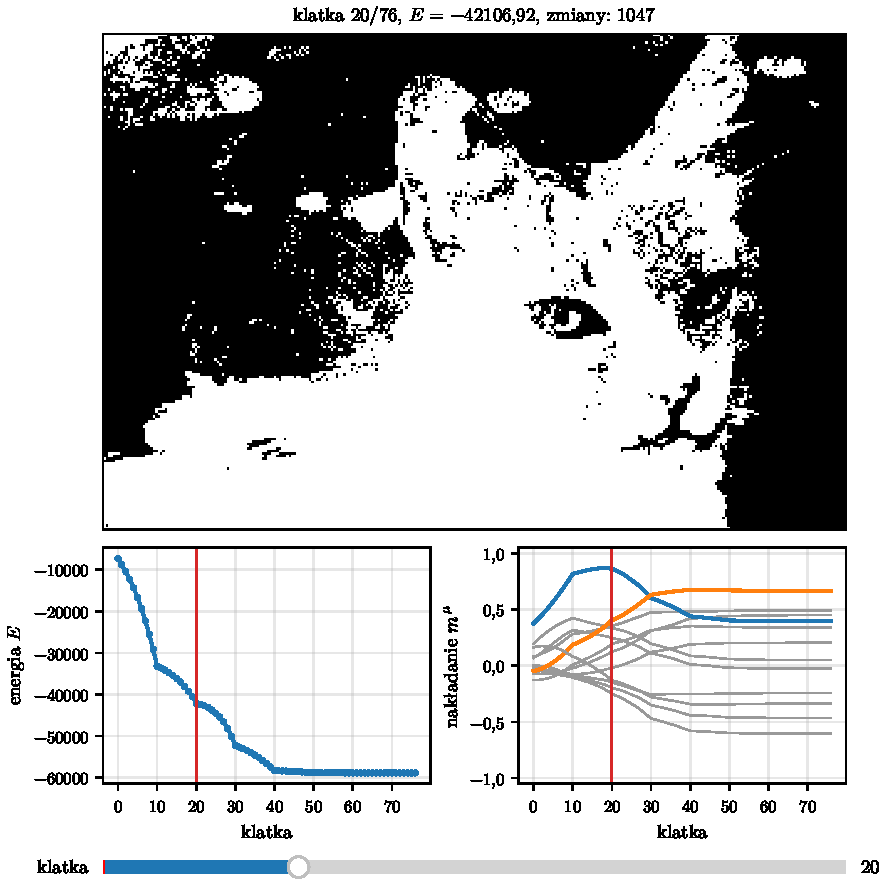
\includegraphics[width=0.8\textwidth]{13-occlusion/figures/viewer-occlusion-hebb.pdf}
    \caption{Przeglądarka kroków dla odtwarzania zdjęcia kota z wejścia, w którym połowę wierszy zasłonięto (reguła Hebba, tryb asynchroniczny, klatka co 6000 aktualizacji). Górny panel: stan w klatce 20 (klatki numerowane od 0 do 76). Lewy dolny wykres: energia w kolejnych klatkach. Prawy dolny wykres: nakładania stanu z wzorcem docelowym (niebieska linia), z wzorcem najbliższym stanowi końcowemu (pomarańczowa linia) i z pozostałymi wzorcami (szare linie). Pionowa linia oznacza bieżącą klatkę.}
    \label{fig:przegladarka}
\end{figure}

\subsection{Powtarzalność}
\label{sec:powtarzalnosc}

Każde uruchomienie, które korzysta z liczb losowych, ma w pliku konfiguracji jawne ziarno generatora \texttt{ChaCha8Rng}. Uszkodzenie wejścia i kolejność aktualizacji korzystają z dwóch osobnych strumieni tego generatora, więc zmiana trybu nie zmienia uszkodzonego wejścia. W eksperymentach z wieloma próbami ziarno każdej próby to pierwsze 8 bajtów skrótu SHA-1 tekstu złożonego z ziarna eksperymentu, nazwy zbioru, rodzaju i poziomu uszkodzenia, numeru wzorca i numeru próby. Ziarno nie zależy od reguły uczenia ani trybu, dlatego obie reguły i oba tryby są porównywane na tych samych wejściach. Każdą próbę można powtórzyć pojedynczym odtwarzaniem z jej ziarnem. Wyniki nie zależą od liczby wątków, a obok wyników zapisywana jest pełna konfiguracja i wersja programu.
